\documentclass[a4paper]{article}
\usepackage{german}
\usepackage[utf8]{inputenc}

\usepackage{pgfplots}
\usepackage{pgfplots.assert}
\usepgflibrary{decorations.pathmorphing}
\usepgfplotslibrary{fillbetween}

\begin{document}
\thispagestyle{empty}
\parindent=0pt
\parskip10pt

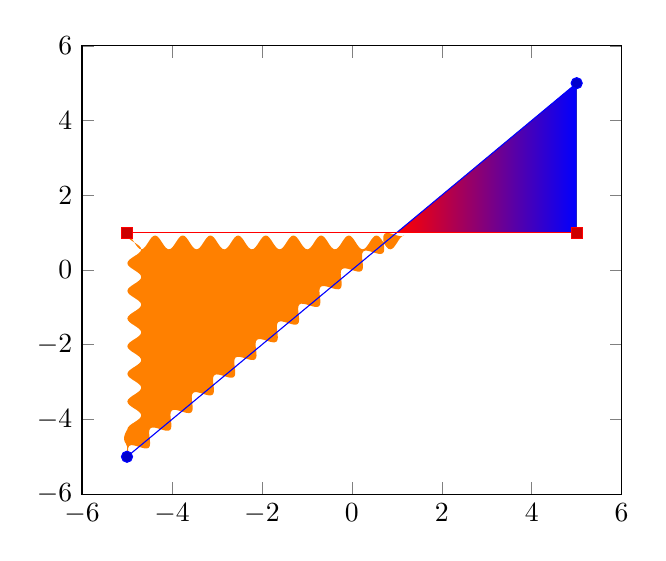
\begin{tikzpicture}
	\begin{axis}[samples=2]
	\addplot+[name path=A] {x};

	\addplot+[name path=B] {1};

	%\tracingmacros=2
	\addplot[decoration=snake] 
		fill between[of=A and B,
			split,
			every segment no 0/.style={fill,orange,decorate},
			every segment no 1/.style={shade,fill,left color=red, right color=blue},
			];
	\end{axis}
\end{tikzpicture}

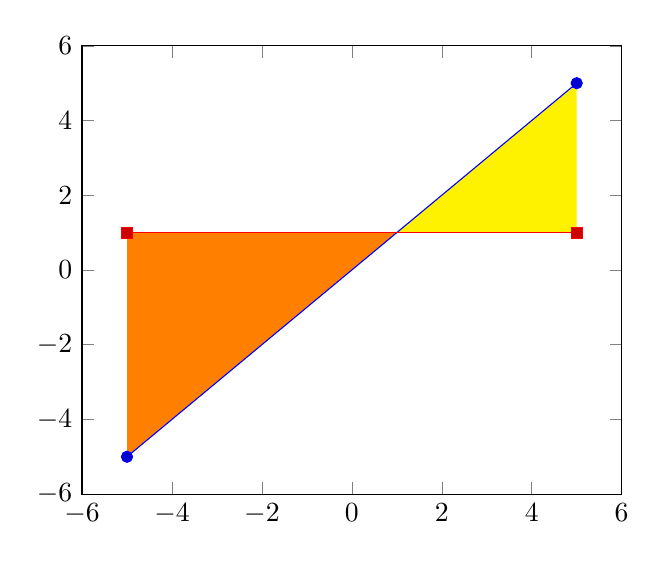
\begin{tikzpicture}
	\begin{axis}[samples=2]
	\addplot+[name path=AA] {x};

	\addplot+[name path=BB] {1};

	%\tracingmacros=2
	\addplot[black]
		fill between[of=AA and BB,
			split,
			every even segment/.style={orange},
			every odd segment/.style={yellow},
			];
	\end{axis}
\end{tikzpicture}



\end{document}

